\documentclass[conference]{IEEEtran}
\IEEEoverridecommandlockouts

\usepackage{cite}
\usepackage{amsmath,amssymb,amsfonts}
\usepackage{algorithm}
\usepackage{algpseudocode}
\usepackage{graphicx}
\usepackage{textcomp}
\usepackage{xcolor}
\usepackage{booktabs}
\usepackage{multirow}
\usepackage{siunitx}
\usepackage{caption}
\usepackage{subcaption}
\usepackage{enumitem}
\usepackage{hyperref}

\renewcommand{\arraystretch}{1.05}

\def\BibTeX{{\rm B\kern-.05em{\sc i\kern-.025em b}\kern-.08em
    T\kern-.1667em\lower.7ex\hbox{E}\kern-.125emX}}

\begin{document}

\title{Object Localization in 3D Semantic Maps via Cluster Bearing and Monocular Distance}

\author{
\IEEEauthorblockN{Author Name}
\IEEEauthorblockA{\textit{Affiliation} \\
\textit{Organization}\\
City, Country \\
email address}
}

\maketitle

\begin{abstract}
Localizing objects in a 3D semantic map for indoor autonomous delivery robots is commonly solved using stereo cameras, RGB-D or LiDAR sensors, or camera-based triangulation methods that depend on the pose odometry of each frame. This paper presents an alternative approach that uses only a low-cost monocular camera (ESP32-CAM), where accuracy comes from algorithm design rather than hardware upgrades. The bearing of the target object is computed from a semantic point cluster --- MapAnything reconstructs the point cloud, YOLO11n attaches the class label, and DBSCAN performs clustering --- with the result transformed into real-world coordinates using the Umeyama algorithm, fitted once over the entire camera trajectory. Distance is estimated from a single frame using the YOLO bounding-box height together with basic geometric principles. Experiments were conducted over sixteen independent capture sessions at three ground-truth distances. At \SI{3}{\meter} and \SI{5}{\meter} the mean error stays under $2\%$, with standard deviations of \SI{0.19}{\meter} and \SI{0.22}{\meter}; at \SI{7}{\meter} a systematic bias of about $-11\%$ appears, but the standard deviation is only \SI{0.07}{\meter}, indicating that the error is dominated by a calibratable bias rather than random noise.
\end{abstract}

\begin{IEEEkeywords}
3D semantic map, object localization, MapAnything, YOLO, autonomous delivery robot, global fit Umeyama, monocular distance estimation
\end{IEEEkeywords}

% =====================================================================
\section{Introduction}
% =====================================================================

The indoor autonomous delivery robot needs to construct and maintain a semantic 3D map to understand object localization and reference points— the object to be delivered, as well as fixed objects such as plant pots, tables, and chairs that can serve as reference points for navigation. A typical pipeline that combines three components  : (i) a 2D detection model (YOLO) that runs on each frame, (ii) a monocular 3D reconstruction model, and (iii) a mechanism for determining the absolute position of objects in the real world, often depends on information from localizing odometry of the robot.

The real-world deployment with low-cost hardware and odometry that accumulates errors over time raises a fundamental question: what really determines the accuracy, and what can we do to improve confidence under limited resources? On the robot Hawkbot (ROS2 Jazzy) equipped with the camera ESP32-CAM, we realize that methodologies that depend on pose odometry of every single frame are sensitive to local noise. The paper presents another methodology: combining orientation, calculated from semantic clustering of objects in MapAnything, with distance estimated from a monocular image, rather than relying on odometry. All sensors include only a low-cost monocular camera — it does not use stereo, RGB-D, or LiDAR; the accuracy mainly comes from algorithm design. The methodology is validated over sixteen independent sessions at three distances (\SI{3}{\meter}, \SI{5}{\meter}, \SI{7}{\meter}), showing stable and consistent results.

% =====================================================================
\section{Related works}
% =====================================================================

The slam systems such as ORB-SLAM~\cite{7219438} optimize camera pose and structure through bundle adjustment and loop closure; the semantic SLAM systems such as SemanticFusion~\cite{7989538}, Kimera~\cite{9196885} extend this approach by attaching class labels to the geometric map in real time. This requires online pose optimization~\cite{7747236}, which is not suitable for the limited computational resources of edge devices used in this research. (Section~\ref{sec:hw-limits}).

Detecting objects on YOLO~\cite{7780460,yolo11}; other methods such as Faster R-CNN~\cite{7485869} or DETR~\cite{carion2020detr} can achieve higher accuracy, but are heavier. With 3D reconstruction using monocular camera images, these direct inference models such as (feed-forward) MapAnything~\cite{mapanything}, Depth Anything~\cite{10657693}, and MiDaS~\cite{9178977} replace the traditional pipeline SfM/MVS with a single inference pass, without multiview camera calibration.

To transform between intrinsic space of the reconstruction model and real-world space from odometry, the Umeyama algorithm~\cite{88573} is classical method for registering fixed point with unknown scale, it is often combined ICP~\cite{121791} for local alignment; DBSCAN~\cite{dbscan} clusters points in the map without requiring to know the number of clusters in advance, making it suitable for separating semantic classes from label noise (Algorithm~\ref{alg:labeling}).

Unlike the approaches above, the method used in the paper does not optimize pose online or perform triangulation for each frame; it separates orientation signals and distance (single-image) from pose odometry for each frame — it is suitable for the post-processing constraint and low-cost hardware of the Hawkbot base.

% =====================================================================
\section{Methodology}
% =====================================================================

\subsection{Hardware}

The entire system is built from popular hardware, low-cost (Table~\ref{tab:hw-specs}) — Not using camera stereo, RGB-D sensor, or LiDAR. This choice makes accuracy mainly depend on algorithm design, rather than on sensor quality.

\begin{table}[t]
\centering
\small
\caption{System configuration}
\label{tab:hw-specs}
\begin{tabular}{@{}p{1.7cm}p{5.4cm}@{}}
\toprule
\textbf{Components} & \textbf{Configurations} \\
\midrule
Robot & Hawkbot, ROS2~\cite{ros} Jazzy (container \texttt{hawkbot-bringup}) \\
Camera & ESP32-CAM, QVGA resolution ($320\times240$ px) \\
Odometry & \texttt{nav\_msgs/Odometry}, topic \texttt{/odom} \\
Processing & remote GPU server, connected through a local network \\
Detection & YOLO11n~\cite{7780460,yolo11} (nano), trained on the COCO-80 dataset \\
3D reconstruction & MapAnything~\cite{mapanything} (\texttt{facebook/map-anything}) \\
\bottomrule
\end{tabular}
\end{table}

Camera intrinsic matrix $K$ (Calibration using checkerboard pattern, 74/75 valid images, with an average reprojection error of 0.12 pixel):
\[
K = \begin{bmatrix}
428.72 & 0 & 148.61 \\
0 & 427.60 & 126.02 \\
0 & 0 & 1
\end{bmatrix}
\label{tab:intrinsics}
\]

\subsection{Current hardware limitations}
\label{sec:hw-limits}

\textbf{Camera resolution.} The camera ESP32-CAM is configured at QVGA to ensure sufficient bandwidth for image transmission and a stable frame rate. This low resolution significantly limits the angular localization accuracy of any method based on pixel positions. When evaluating the use of the localization marker ArUco~\cite{GARRIDOJURADO20142280} \SI{15}{\centi\meter}(Section~\ref{sec:hw-alternatives}), a one-degree error in estimating the marker angle, at a distance of more than two meters, can correspond to a real-world positional error of up to several tens of centimeters.

\textbf{Computational capacity.} ESP32-CAM does not perform computer vision processing locally; all Yolo and MapAnything inference runs on a remote GPU server. The current pipeline operates offline in post-processing rather than as an online SLAM system; adding an online correction mechanism, such as loop closure and pose-graph optimization, requires computational resources the current platform cannot provide. 

The two limitations above are reasons why this research focuses on finding a software methodology; it does not require upgrading hardware- the methodology, which combines semantic clusters and single image distance(Section~\ref{sec:math}) — rather than adding more hardware- is proposed as an improvement in future development (Section~\ref{sec:limitations}).

\subsection{Pipeline Architecture}

Three main processing block of pipeline: \textbf{(i) 3D reconstruction} using MapAnything (S3), \textbf{(ii) Attaching semantic class label YOLO on 3D map} to have semantic point cloud (S4), and \textbf{(iii) Estimating single-image distance} (S7) — two signals (ii) and (iii) then is combined without triangulation through many frames.

\begin{enumerate}[label=\textbf{S\arabic*.},leftmargin=*,itemsep=0.05em,topsep=0.1em,parsep=0pt]
    \item \textbf{Collection:} Robot moves independently; the camera continuously captures images ($\sim$1 frame/second), recording localization/ odometry orientation for each frame into \texttt{poses.json}.
    \item \textbf{Priority frame selection:} Running YOLO on the overall original frame, selecting up to 130 frames containing the target object, and uniformly sampling across each visit.
    \item \textbf{3D reconstruction:} Running MapAnything~\cite{mapanything} on selected frames, reconstructing a pure geometric point cloud and the intrinsic camera trajectory.
    \item \textbf{Attaching semantic class label (YOLO $\to$ 3D):} Running YOLO on each frame, attaching COCO class label for each 3D point in bounding box (Algorithm~\ref{alg:labeling}), creates \emph{semantic point cloud}.
    \item \textbf{Global fit:} Umeyama fit between MapAnything trajectory and odometry trajectory $\to$ $(s, R, \mathbf{t})$, calculated once for overall session.
    \item \textbf{Object orientation:} Filtering point belonging to the target class label, DBSCAN clustering~\cite{dbscan}, Selecting max cluster center; apply global fit to inference the orientation.
    \item \textbf{Object distance:} on the only frame, Single-image estimation from the YOLO bounding box height, real height, and camera focal length (\S~\ref{sec:math}).
    \item \textbf{Combining:} localization = reference camera localization + orientation $\times$ distance.
\end{enumerate}

Algorithm ~\ref{alg:labeling} describes the mechanism for attaching semantic class labels for 3D points at S4 — basic for determining target clusters at S6.

\begin{algorithm}[!ht]
\footnotesize
\caption{Attaching semantic class labels for 3D point cloud}
\label{alg:labeling}
\begin{algorithmic}[1]
\Require Selected frame $\{I_1, \dots, I_n\}$; MapAnything $\mathcal{M}$; YOLO $\mathcal{Y}$
\Ensure labeled Point cloud $\mathcal{P} = \{(\mathbf{x}_j, l_j)\}$
\State $\mathcal{P} \gets \emptyset$
\For{$i \gets 1$ \textbf{to} $n$}
    \State $(D_i, K_i, T_i, M_i) \gets \mathcal{M}(I_i)$ \Comment{depth, K, pose, mask}
    \State $\mathbf{P}_i \gets \textsc{DepthToWorld}(D_i, K_i, T_i)$
    \State $B_i \gets \mathcal{Y}(I_i)$ \Comment{$(l, \text{bbox}, \text{conf})$, Filtering by conf}
    \For{each pixel $(u, v)$, $M_i(u, v) = \text{true}$}
        \State $l \gets -1$ \Comment{default: background}
        \For{each $(l', \text{bbox}, \text{conf}) \in B_i$}
            \If{$(u, v) \in \text{bbox}$}
                \State $l \gets l'$; \textbf{break}
            \EndIf
        \EndFor
        \State $\mathcal{P} \gets \mathcal{P} \cup \{(\mathbf{P}_i(u, v),\ l)\}$
    \EndFor
\EndFor
\State \Return $\mathcal{P}$
\end{algorithmic}
\end{algorithm}

\textbf{Limitations of labeling mechanism.} The check at line 8 only determines whether a pixel is inside the 2D YOLO \emph{bounding box}, not semantic segmentation at the pixel level. Background points or other objects falling inside the bounding box may also be incorrectly labeled. This is why the DBSCAN step at S6 is necessary: the densest point cluster — corresponding to the actual object observed consistently from multiple views — is separated from scattered noise points.

\subsection{Formula}
\label{sec:math}

\textbf{Global fit (Umeyama fit)~\cite{88573}.} Let $\{\mathbf{q}_k\}$ denote camera positions from MapAnything (projected onto the horizontal plane) and $\{\mathbf{p}_k\}$ denote odometry positions, respectively. The Umeyama algorithm finds $s \in \mathbb{R}$, $R \in SO(2)$, and $\mathbf{t}$ that minimize:
\begin{equation}
(s^*, R^*, \mathbf{t}^*) = \operatorname*{arg\,min}_{s, R, \mathbf{t}} \sum_k \left\lVert \mathbf{p}_k - \left(s R \mathbf{q}_k + \mathbf{t}\right) \right\rVert^2
\end{equation}
It is solved using SVD on the cross-covariance matrix between the two centered point sets. The point $\mathbf{x}_{\text{raw}}$ in the MapAnything is transformed into real-world space as: $\mathbf{x}_{\text{real}} = s^* R^* \mathbf{x}_{\text{raw}} + \mathbf{t}^*$.

\textbf{Orientation.} With $\mathbf{c}_{\text{raw}}$ is centroid of the largest semantic point cluster and $\mathbf{o}$ is reference camera position:
\begin{equation}
\hat{\mathbf{b}} = \frac{\left(s^* R^* \mathbf{c}_{\text{raw}} + \mathbf{t}^*\right) - \mathbf{o}}{\left\lVert \left(s^* R^* \mathbf{c}_{\text{raw}} + \mathbf{t}^*\right) - \mathbf{o} \right\rVert}
\end{equation}

\textbf{Single-image distance.} With bbox height $h_{\text{px}}$, real height  $H$, focal length $f_y$:
\begin{equation}
d = \frac{f_y \cdot H}{h_{\text{px}}}, \qquad
\mathbf{x}^* = \mathbf{o} + d \, \hat{\mathbf{b}}
\end{equation}

\textbf{Distance-size ambiguity.} The formula (3) prior assumption $H$ for the target class. If there are two objects of the same class with known actual height $H_1 \neq H_2$, placed at two distances $d_1, d_2$ such that
\begin{equation}
\frac{H_1}{d_1} = \frac{H_2}{d_2} \;\left(= \frac{h_{\text{px}}}{f_y}\right),
\end{equation}
Two objects show the same $h_{\text{px}}$ on image and the formula (3) does not distinguish — this is distance- size ambiguity which is typical of monocular camera, it is not solved by only formula, geometric or deep learning model (Section~\ref{sec:global-fit-stable} Further analysis of why Mapanything's depth inference does not automatically overcome this limitation. The clustering step DBSCAN at S6, prioritizing the densest and persistent point cluster across multiple frames, reducing the risk of confusing it with false objects that appear only briefly, but does not eliminate confusion between two same class entities  — the method implicitly assumes that the environment contains only one instance of the target class, which is consistent with the current experimental setup (Section~\ref{sec:limitations}).

None of quantities above depend on the pose odometry of a single frame, except for $\mathbf{o}$ (reference results) — the alignment uses entire trajectory, while the distance estimation does not use odometry Figure~\ref{fig:pipeline-new} is a visual overview of entire localization pipeline that described above, include three blocks (i) 3D reconstruction, (ii) Attaching YOLO semantic labels, and (iii) distance estimation.

\begin{figure*}[t]
\centering
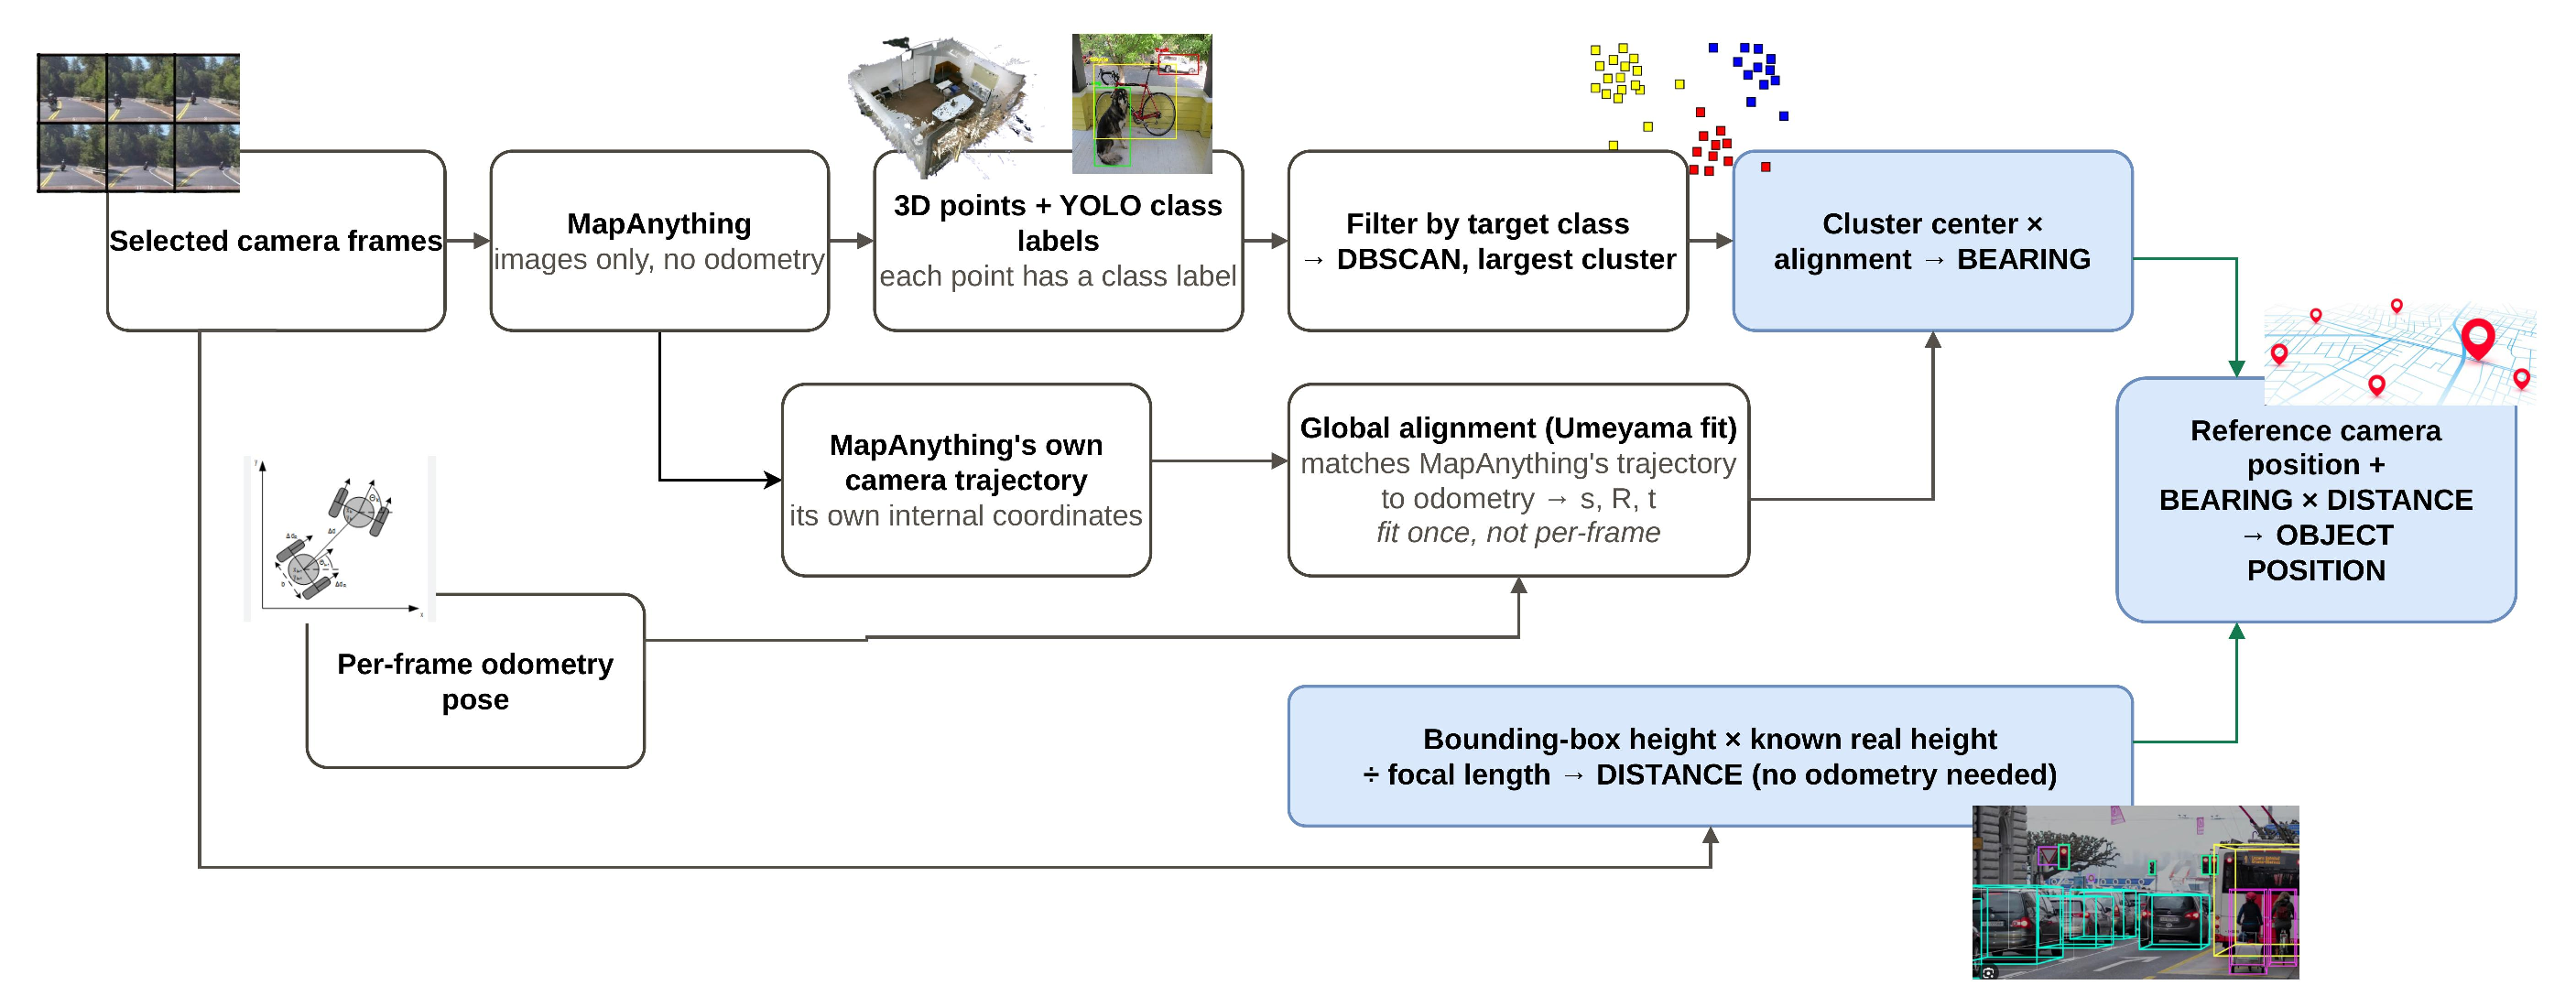
\includegraphics[width=0.72\textwidth]{paper_figs/hinh1_pipeline.drawio.pdf}
\caption{Object localization pipeline combining bearing estimated from MapAnything semantic point clusters with monocular distance estimation.}
\label{fig:pipeline-new}
\end{figure*}


% =====================================================================
\section{Experimental Results}
\label{sec:semantic-bearing}
% =====================================================================

With each capture session, three processing blocks at Section~\ref{sec:math} are performed sequentially: \textbf{(i)} Reconstructing a 3D map using MapAnything, \textbf{(ii)} Attaching YOLO labels on each 3D point to have semantic point cloud, and \textbf{(iii)} Estimating single-image distance — two orient signals (from (ii)) and distance (from (iii)) then combined to create localization. The method is validated at six independent capture session at \SI{3.00}{\meter} (measured using a measuring tape.), Each time, the robot observes the plant pot from a different trajectory. To evaluate the stability when extending the range, the process is repeated at \SI{5}{\meter} and \SI{7}{\meter}, five sessions at each level, combining with \SI{3}{\meter} at Table~\ref{tab:semantic-bearing-results} and analyzed separately at Section~\ref{sec:distance-eval}. Figure~\ref{fig:room-scan} illustrates the experimental environment from a single scan of the entire room. (detail at Section~\ref{sec:room-scan}).

\begin{figure*}[t]
\centering
\begin{subfigure}[b]{0.46\textwidth}
\centering
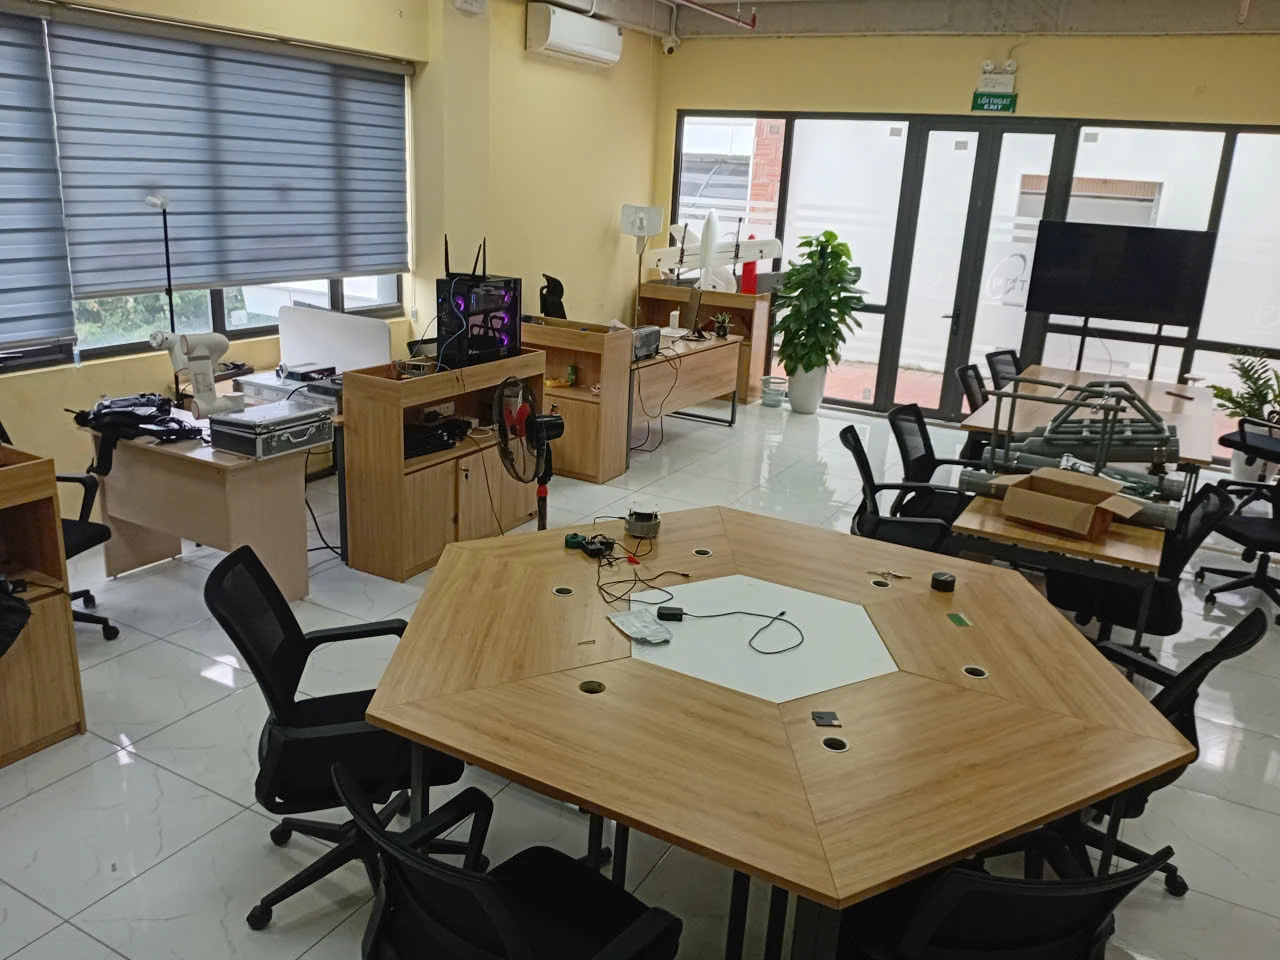
\includegraphics[height=3.2cm,keepaspectratio]{paper_figs/room_scan_photo.png}
\caption{Real-world captured image}
\end{subfigure}
\hspace{0.6em}
\begin{subfigure}[b]{0.46\textwidth}
\centering
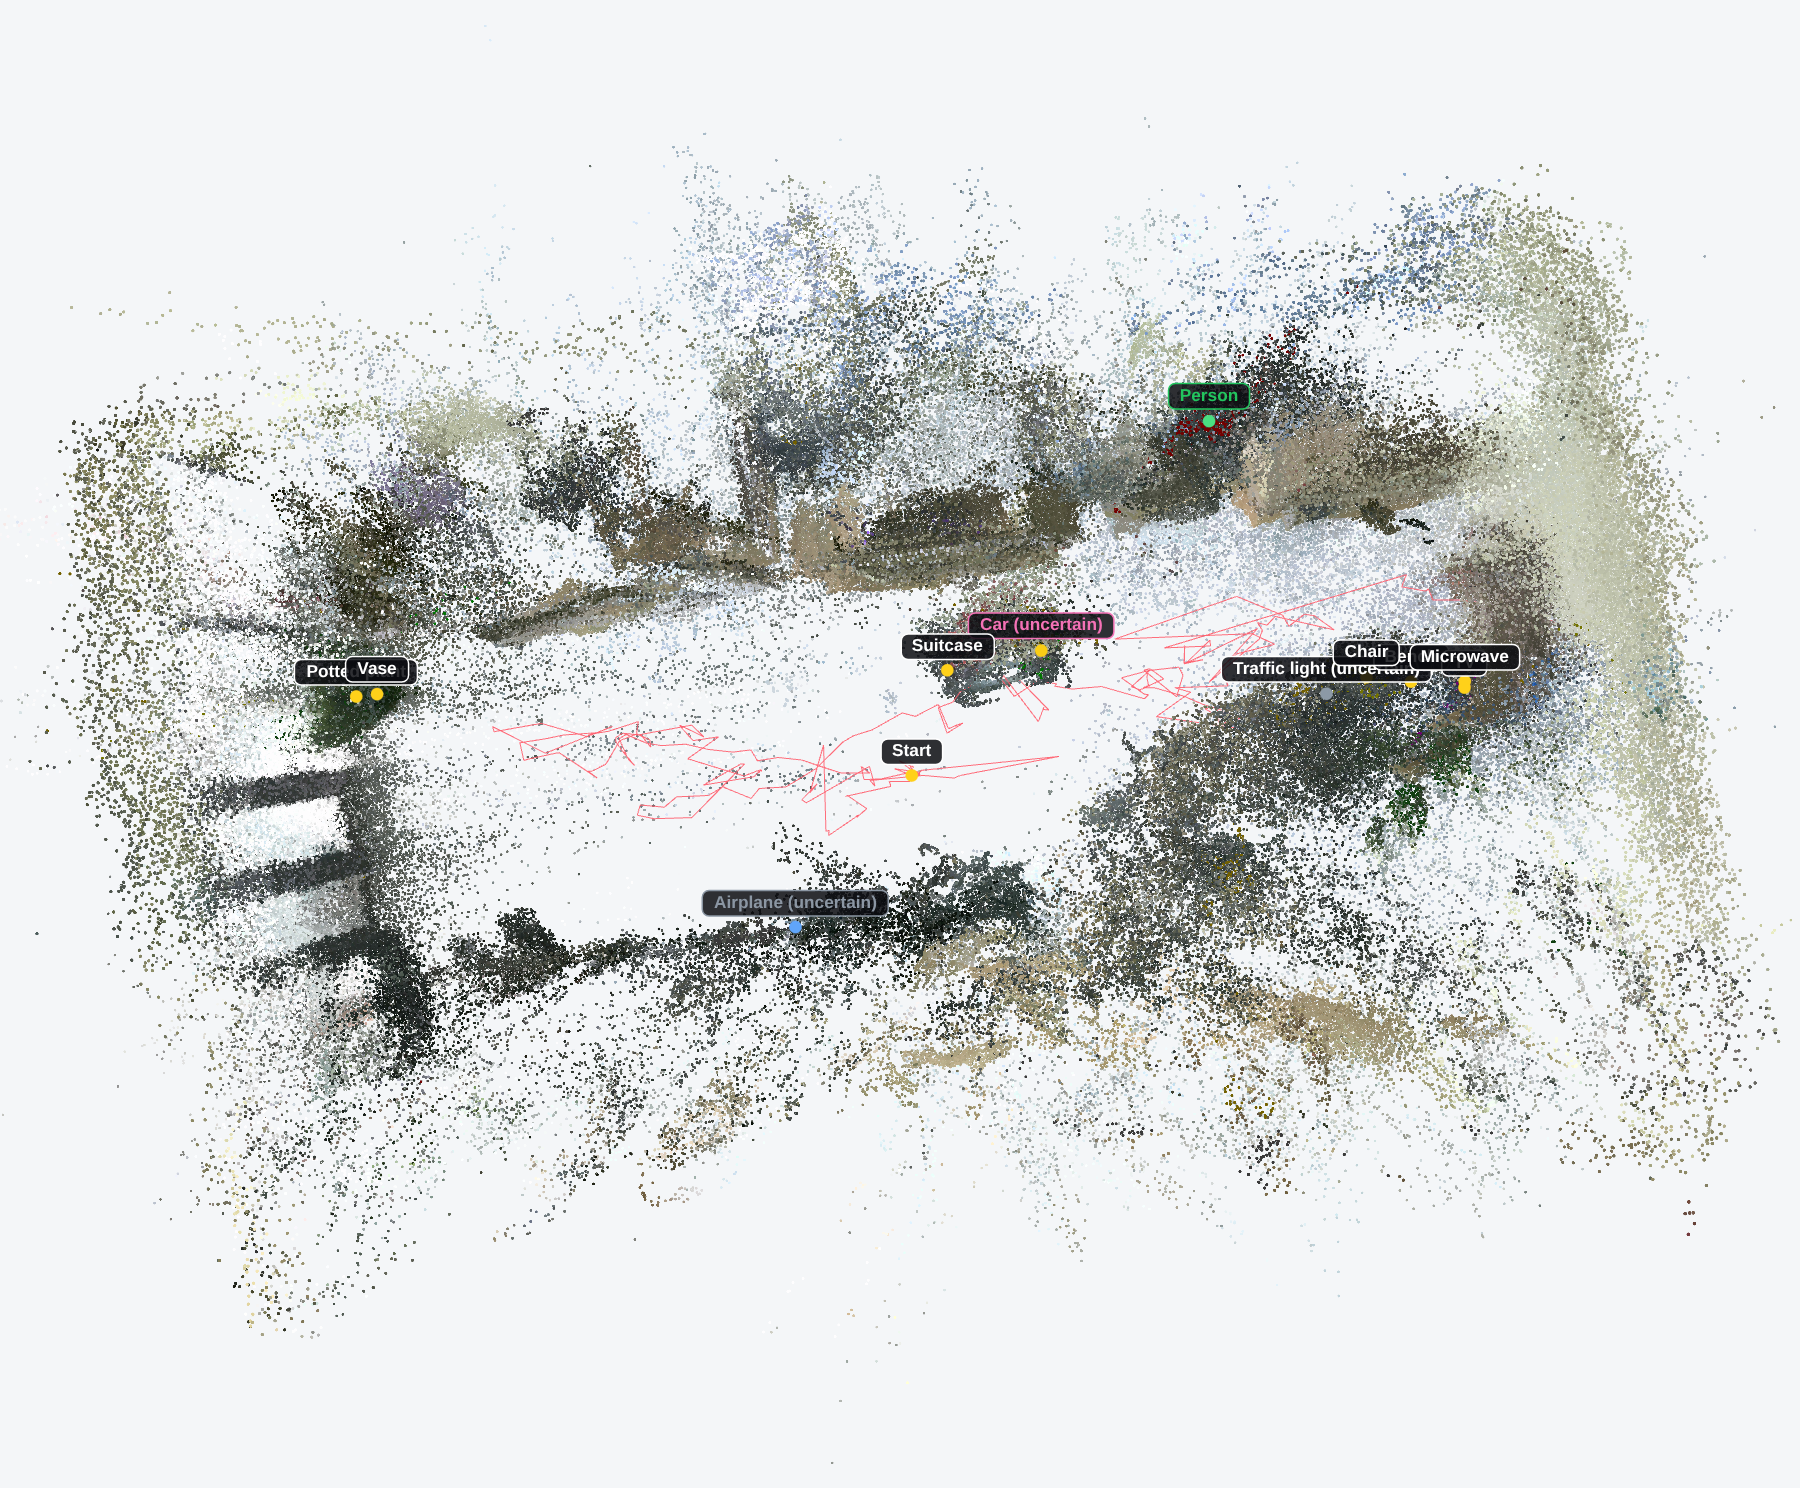
\includegraphics[height=3.2cm,keepaspectratio]{paper_figs/room_scan_topdown.png}
\caption{Point map (top view, aligned with the direction of the real-world image))}
\end{subfigure}
\caption{Full-room scan: real-world image (left) and 3D point map reconstructed from 239 frames (right). Yellow marker: centroid of the largest point cluster; red line: robot trajectory.}
\label{fig:room-scan}
\end{figure*}

\begin{table*}[t]
\centering
\small
\caption{Plant localization results at three real-world distances
(\SI{3}{\meter}: six capture sessions; \SI{5}{\meter} and \SI{7}{\meter}:
five sessions each), together with input quality indicators}
\label{tab:semantic-bearing-results}
\begin{tabular}{@{}clccccc@{}}
\toprule
\textbf{Real-world} & \textbf{Capture} & \textbf{Estimated} & \textbf{Error} & \textbf{YOLO} & \textbf{BBox height} & \textbf{Semantic cluster} \\
\textbf{distance} & \textbf{session} & \textbf{distance} & \textbf{w.r.t. ground truth} & \textbf{confidence} & \textbf{(px)} & \textbf{points} \\
\midrule
\multirow{6}{*}{\SI{3}{\meter}}
 & 1 & \SI{2.77}{\meter} & $-7.6\%$ & 0.63 & 192.9 & 29\,841 \\
 & 2 & \SI{2.76}{\meter} & $-8.1\%$ & 0.90 & 193.9 & 29\,992 \\
 & 3 & \SI{3.13}{\meter} & $+4.2\%$ & 0.78 & 170.9 & 29\,974 \\
 & 4 & \SI{3.08}{\meter} & $+2.6\%$ & 0.65 & 173.6 & 29\,773 \\
 & 5 & \SI{3.26}{\meter} & $+8.5\%$ & 0.76 & 164.2 & 29\,913 \\
 & 6 & \SI{3.12}{\meter} & $+3.9\%$ & 0.76 & 171.4 & 30\,000 \\
\cmidrule(l){2-7}
 & \multicolumn{1}{l}{Mean} & \SI{3.02}{\meter} &
 \multicolumn{4}{r}{Std. dev. \SI{0.19}{\meter}, mean error $+0.6\%$ (absolute mean $6.2\%$)} \\
\midrule
\multirow{5}{*}{\SI{5}{\meter}}
 & 1 & \SI{4.49}{\meter} & $-10.2\%$ & 0.81 & 119.1 & 29\,606 \\
 & 2 & \SI{5.07}{\meter} & $+1.4\%$  & 0.74 & 105.4 & 29\,984 \\
 & 3 & \SI{5.00}{\meter} & $+0.0\%$  & 0.85 & 106.9 & 25\,826 \\
 & 4 & \SI{5.06}{\meter} & $+1.2\%$  & 0.82 & 105.6 & 25\,932 \\
 & 5 & \SI{5.01}{\meter} & $+0.3\%$  & 0.75 & 106.6 & 22\,543 \\
\cmidrule(l){2-7}
 & \multicolumn{1}{l}{Mean} & \SI{4.93}{\meter} &
 \multicolumn{4}{r}{Std. dev. \SI{0.22}{\meter}, mean error $-1.5\%$ (absolute mean $2.6\%$)} \\
\midrule
\multirow{5}{*}{\SI{7}{\meter}}
 & 1 & \SI{6.21}{\meter} & $-11.3\%$ & 0.85 & 86.1 & 29\,742 \\
 & 2 & \SI{6.22}{\meter} & $-11.1\%$ & 0.51 & 85.9 & 29\,588 \\
 & 3 & \SI{6.17}{\meter} & $-11.9\%$ & 0.73 & 86.6 & 30\,000 \\
 & 4 & \SI{6.34}{\meter} & $-9.4\%$  & 0.71 & 84.3 & 29\,662 \\
 & 5 & \SI{6.13}{\meter} & $-12.4\%$ & 0.82 & 87.2 & 29\,933 \\
\cmidrule(l){2-7}
 & \multicolumn{1}{l}{Mean} & \SI{6.21}{\meter} &
 \multicolumn{4}{r}{Std. dev. \SI{0.07}{\meter}, mean error $-11.2\%$} \\
\bottomrule
\end{tabular}
\end{table*}
\subsection{Quantitative results}

Table~\ref{tab:semantic-bearing-results} The results at each session are summarized, together with  detection/clustering quality indicators : the YOLO detection confidence at frame which used to estimate distance, the height of bounding box respectively, the number of points which in the largest semantic cluster used to inference orientation.

Six captured sessions show errors in the range $2$--$9\%$ compared to real-world values; no session shows an excessively large error \SI{0.26}{\meter}. Notably, the YOLO confidence varies considerably (0.63--0.90) while the number of semantic cluster points varies at high level ($>$29\,700/30\,000 points, meaning target cluster accounts for more than 99\% of the sampled points) — this shows that the objects are reconstructed by MapAnything  into a contiguous point cluster, with little fragmentation, regardless of the detection confidence.

\textbf{Correlation between input quality indicators and localization error} The Pearson correlation coefficient between YOLO confidence and the absolute error is $r = 0.34$; between the number of clusters and the error $r = 0.20$ — Both correlations are weak and statistically insignificant. with $n=6$. This result is consistent with the theoretical expectation. At section~\ref{sec:global-fit-stable}: the accuracy mainly comes from separating two signals from  pose odometry each frame,rather than coming from high-confidence detection or large semantic cluster.

\begin{figure}[t]
\centering
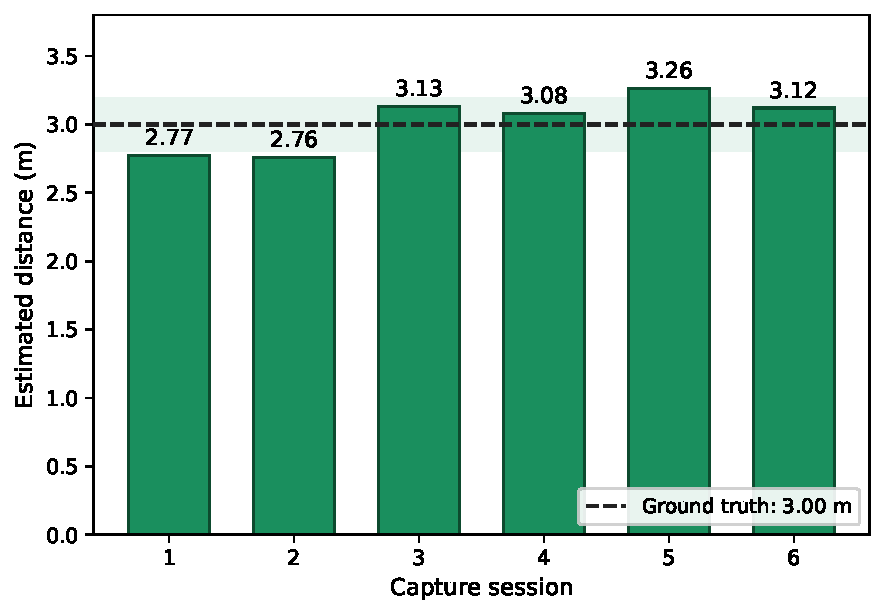
\includegraphics[width=0.85\columnwidth]{paper_figs/fig_results_bar_en.pdf}
\caption{Estimated distances across six capture sessions, compared with the
ground-truth distance of \SI{3.00}{\meter} (dashed line). Shaded region:
$\pm 1$ standard deviation around the mean.}
\label{fig:results-bar}
\end{figure}

\subsection{Visualization on the point map}

Figure~\ref{fig:six-viewers} illustrates localized object positions provided with the robot trajectory on the point cloud map of six captured sessions. Figure~\ref{fig:6cap-3d} visualizes the distribution of estimated distances of six sessions around the ground truth measurements \SI{3.00}{\meter}, showing that the estimates converge around the reference line within the range $\pm 1$ standard deviation. The results of six sessions show average errors of about $6\%$, not clearly depending on trajectory shape (Figure~\ref{fig:six-viewers}) or the 2D detection confidence (Table~\ref{tab:semantic-bearing-results}) — consistent with the argument presented in Section~\ref{sec:global-fit-stable}. Figure~\ref{fig:real-photo} Comparison of the real-world experimental environment with a YOLO11n frame detecting the plant pot.

\begin{figure}[t]
\centering
\begin{subfigure}[b]{0.48\columnwidth}
\centering
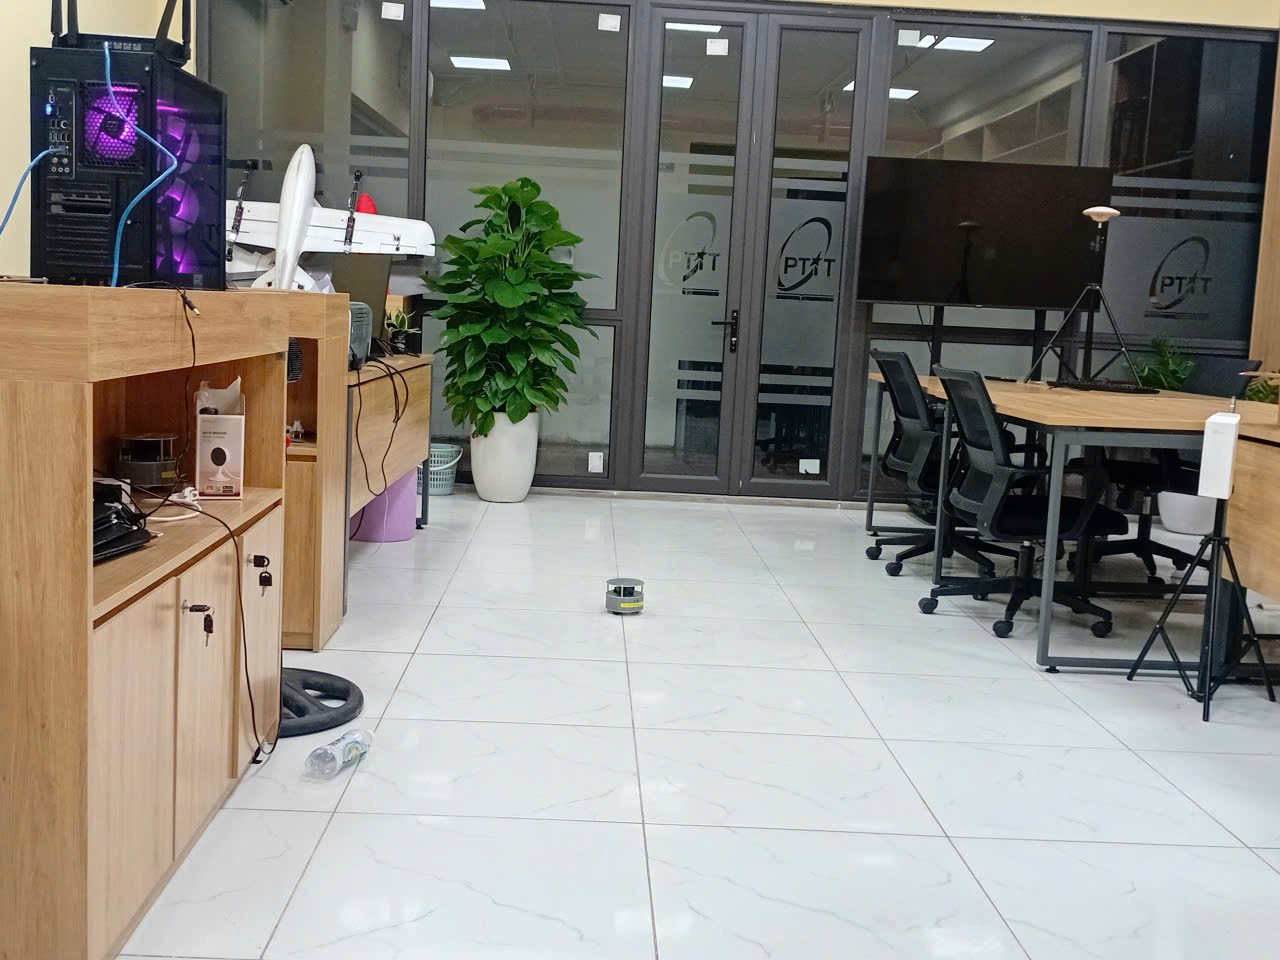
\includegraphics[height=2.1cm,keepaspectratio]{paper_figs/anh_thuc_te.jpg}
\caption{Experimental environment}
\end{subfigure}
\hfill
\begin{subfigure}[b]{0.48\columnwidth}
\centering
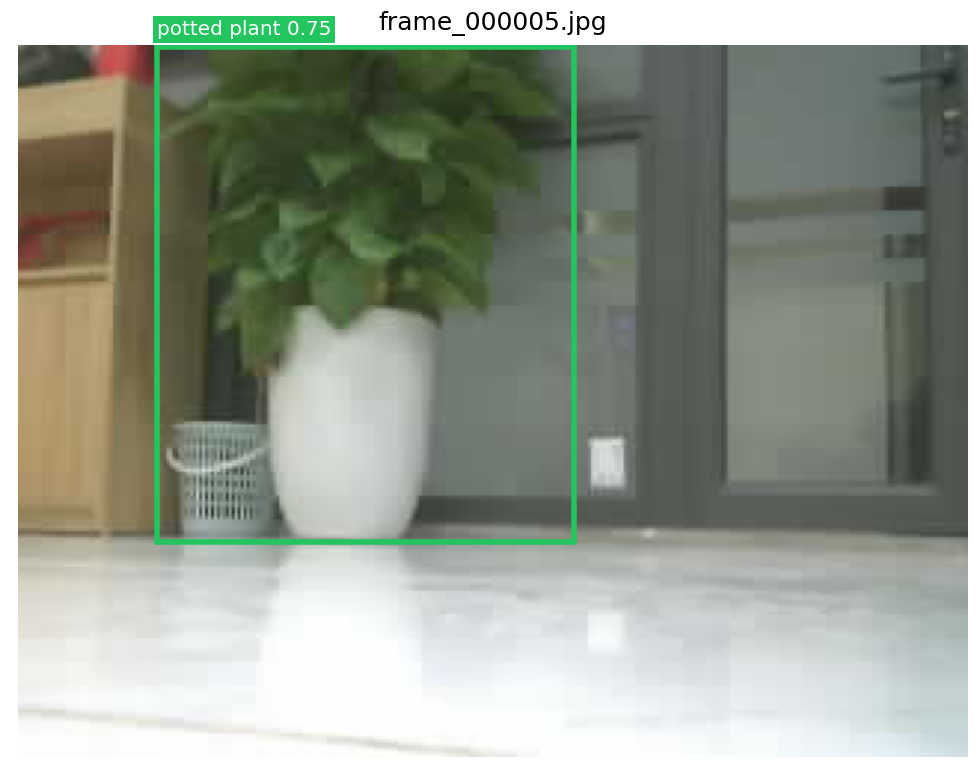
\includegraphics[height=2.1cm,keepaspectratio]{paper_figs/fig_yolo_detection_single.png}
\caption{YOLO11n plant pot detection}
\end{subfigure}
\caption{Real-world experimental environment (left): the Hawkbot robot positioned in the middle of the floor in an office space, with the plant pot as the target object. YOLO11n detection on an ESP32-CAM frame (right), with a confidence score of 0.75.}
\label{fig:real-photo}
\end{figure}

\begin{figure}[t]
\centering
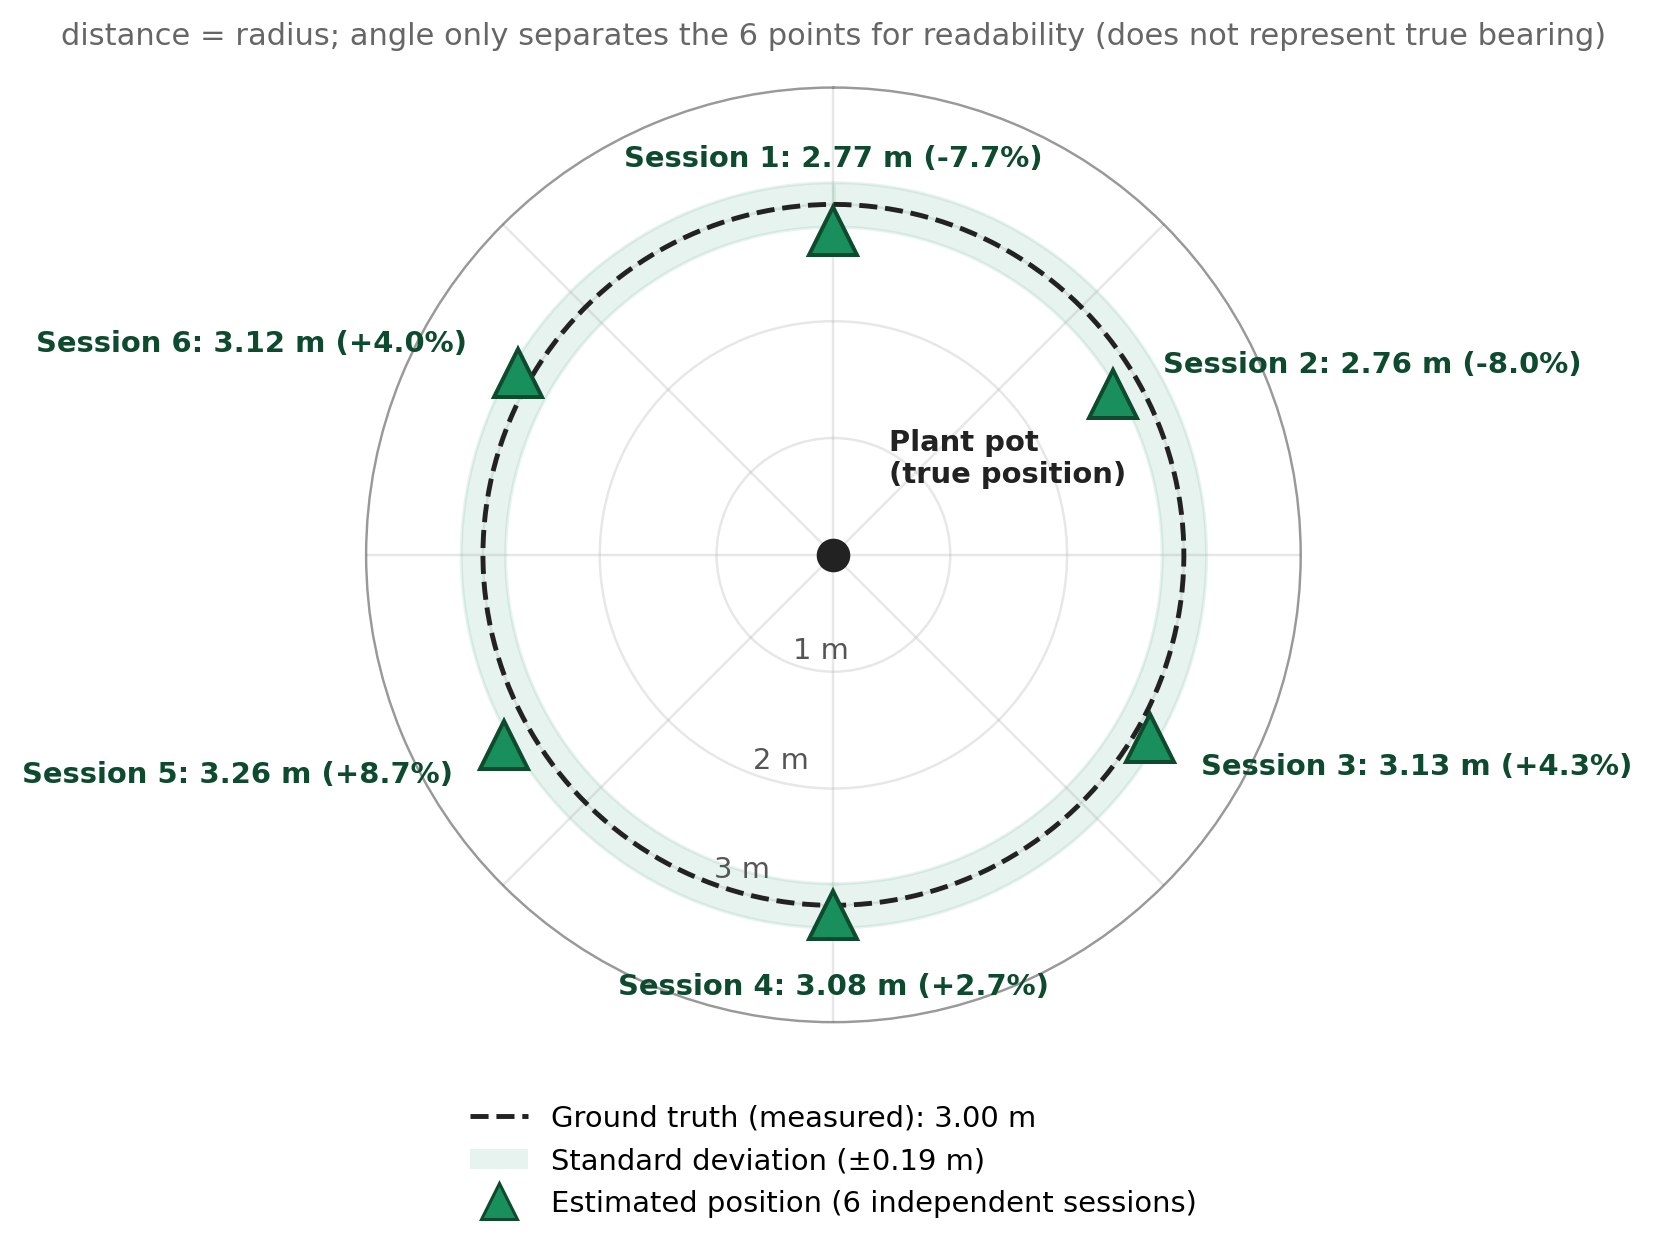
\includegraphics[width=0.72\columnwidth]{paper_figs/figure5.png}
\caption{Distribution of estimated distances across six independent capture sessions around the ground-truth distance of \SI{3.00}{\meter} (dashed circle). Green triangles denote the estimated distance for each session, the black dot at the center indicates the true plant-pot position, and the shaded region represents the $\pm 1$ standard deviation range (\SI{0.19}{\meter}). The angular positions are used only to separate the points for readability and do not represent actual bearing directions.}
\label{fig:6cap-3d}
\end{figure}

\begin{figure*}[t]
\centering
\begin{subfigure}[t]{0.32\textwidth}
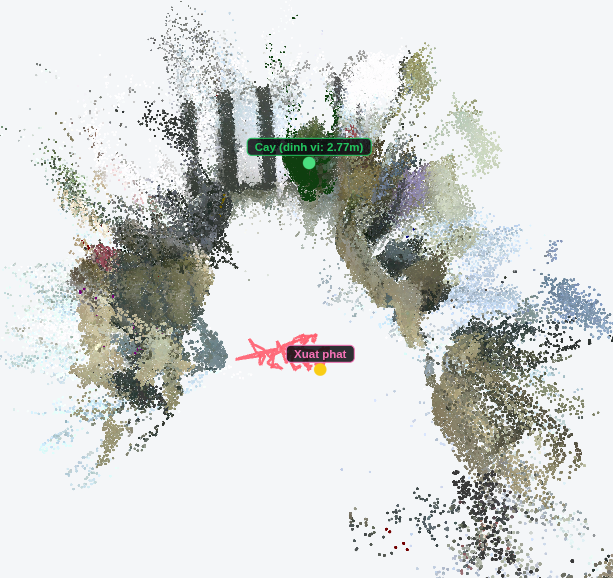
\includegraphics[width=\textwidth]{paper_figs/paperfig_new36.png}
\caption{Session 1 --- \SI{2.77}{\meter}}
\end{subfigure}
\hfill
\begin{subfigure}[t]{0.32\textwidth}
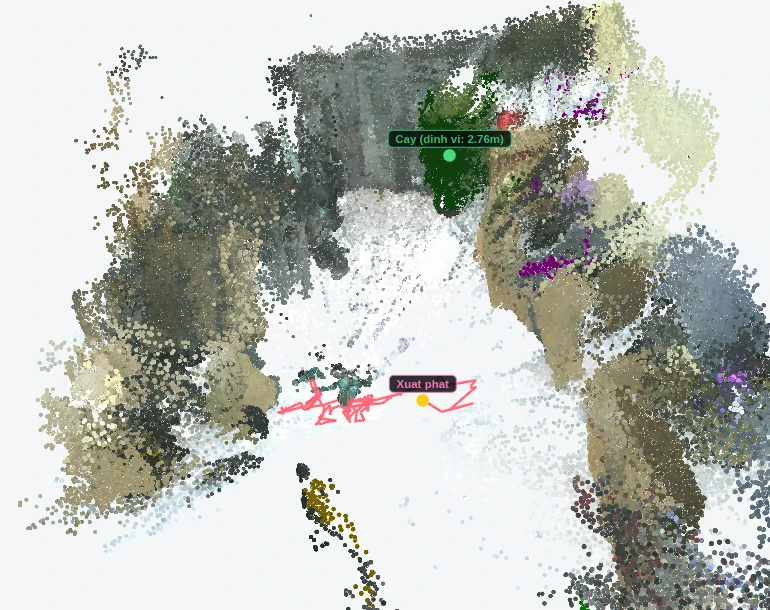
\includegraphics[width=\textwidth]{paper_figs/paperfig_new46.png}
\caption{Session 2 --- \SI{2.76}{\meter}}
\end{subfigure}
\hfill
\begin{subfigure}[t]{0.32\textwidth}
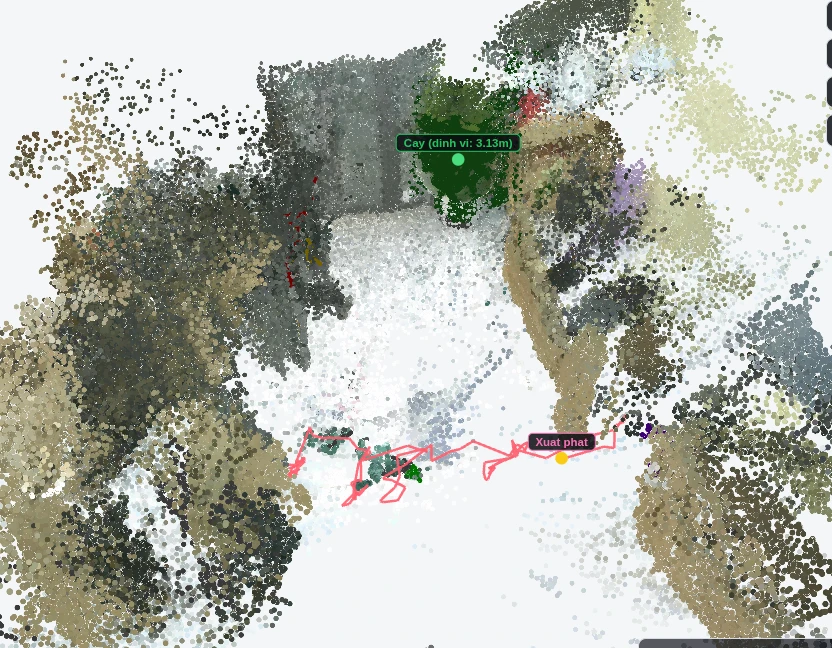
\includegraphics[width=\textwidth]{paper_figs/paperfig_new47.png}
\caption{Session 3 --- \SI{3.13}{\meter}}
\end{subfigure}

\vspace{0.1em}
\begin{subfigure}[t]{0.32\textwidth}
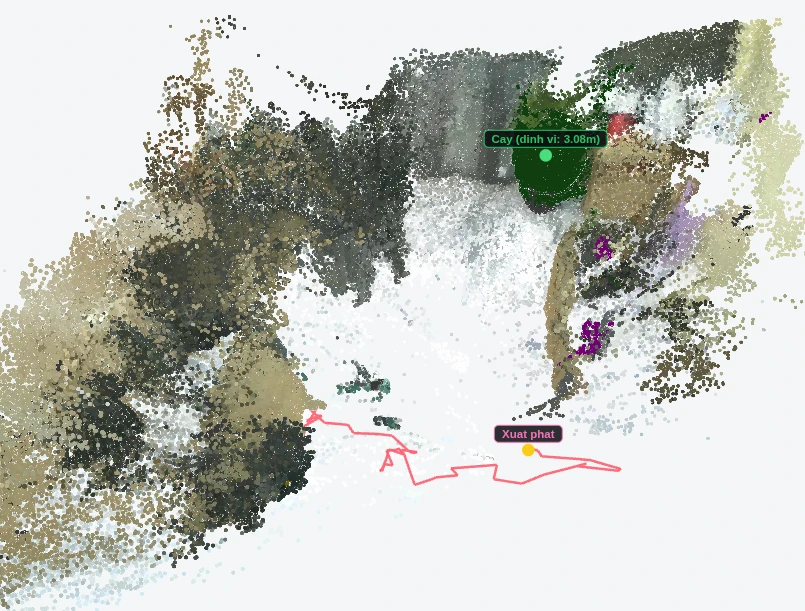
\includegraphics[width=\textwidth]{paper_figs/paperfig_new48.png}
\caption{Session 4 --- \SI{3.08}{\meter}}
\end{subfigure}
\hfill
\begin{subfigure}[t]{0.32\textwidth}
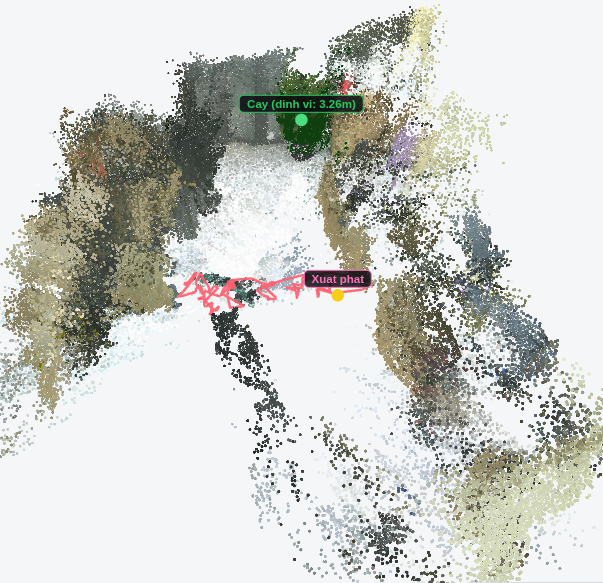
\includegraphics[width=\textwidth]{paper_figs/paperfig_new49.png}
\caption{Session 5 --- \SI{3.26}{\meter}}
\end{subfigure}
\hfill
\begin{subfigure}[t]{0.32\textwidth}
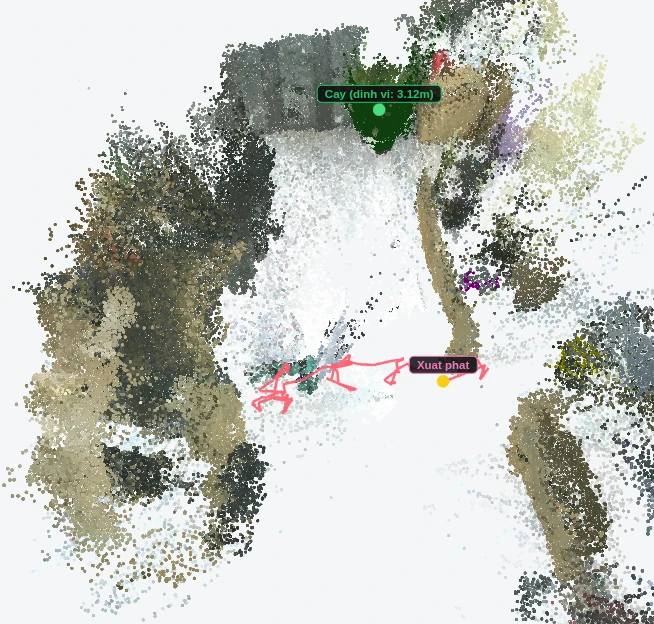
\includegraphics[width=\textwidth]{paper_figs/paperfig_new50.png}
\caption{Session 6 --- \SI{3.12}{\meter}}
\end{subfigure}

\caption{Localized plant-pot position (green marker) and robot trajectory (red line, starting point marked) on the MapAnything point-cloud map for six independent capture sessions.}
\label{fig:six-viewers}
\end{figure*}

\subsection{Extension: Full-room semantic map scanning}
\label{sec:room-scan}

To evaluate scalability of the pipeline beyond the single target localization scenario, we move the robot around the room (239 frames, instead of the 130 frames focused on a single object as in Section~\ref{sec:semantic-bearing}) and run the entire pipeline again for S1--S8 unlimited target semantic classes. The result is a 3D map with 38.8 million points, while YOLO11n attaches 12 different COCO labels. Figure~\ref{fig:room-scan} compares a real-world photograph of the room with the top-down view of the point map.

The reconstructed map accurately preserves the overall shape and layout of the furniture (tables, chairs, cabinets, and the plant pot at their corresponding relative positions). However, due to the QVGA camera combined with the YOLO11n nano model, some detected labels are false positives—for example, ``car'', ``airplane'', and ``traffic light'', which are largely absent from the actual office environment—consistent with the hardware limitations discussed in Section~\ref{sec:hw-limits}. These results demonstrate that the pipeline generalizes well to full-room mapping, although the reliability of semantic labeling remains constrained by the current sensing hardware.

\subsection{Distance-dependent accuracy evaluation}
\label{sec:distance-eval}

The six capture sessions in Section~\ref{sec:semantic-bearing} were all conducted at \SI{3.00}{\meter}. To evaluate whether the method remains accurate at greater target distances, we repeated the B1--B8 procedure, keeping $H=\SI{1.25}{\meter}$ and using the same target plant pot, at two additional distances: five sessions at \SI{5}{\meter} and five sessions at \SI{7}{\meter}, with the results summarized in Table~\ref{tab:semantic-bearing-results}.

The three result groups reveal two distinct error patterns. At \SI{3}{\meter} and \SI{5}{\meter}, the mean error nearly cancels ($+0.6\%$ and $-1.5\%$), but the standard deviations are relatively large (\SI{0.19}{\meter}, \SI{0.22}{\meter}), with individual sessions deviating up to $\pm 10\%$ — characteristic of random noise. At \SI{7}{\meter}, in contrast, the standard deviation is very small (\SI{0.07}{\meter}, less than one-third of the two shorter ranges), yet all five sessions consistently show a $-11\%$ bias, characteristic of a systematic error. Because $d = f_y H / h_{\text{px}}$ gives a proportional relationship between $d$ and $1/h_{\text{px}}$, a constant relative error in $f_y$ (camera calibration) or $H$ (assumed plant-pot height) produces exactly the observed nearly-constant bias. Recalibrating $f_y$ or measuring $H$ more accurately is therefore a direct mitigation (Section~\ref{sec:limitations}).

% =====================================================================
\section{Discussion}
% =====================================================================

\subsection{Why Global Fitting Is More Stable Than Per-Frame Triangulation}
\label{sec:global-fit-stable}

Both signals used by the method avoid dependence on the odometry pose of any single frame. The Umeyama alignment uses the entire camera trajectory, reducing the effect of local pose noise, while the monocular distance depends only on the object's image size and the calibrated camera intrinsics.

\textbf{Empirical validation.} To evaluate whether the direct 3D position from MapAnything could replace the monocular distance, we compute $\lVert (s^*R^*\mathbf{c}_{\text{raw}}+\mathbf{t}^*)-\mathbf{o}\rVert$ for all sixteen sessions without using Eq.~(3). The results are compared with the proposed method in Table~\ref{tab:3d-vs-mono}.


\begin{table}[t]
\centering
\small
\caption{Mean error: monocular distance vs. direct MapAnything 3D position}
\label{tab:3d-vs-mono}
\begin{tabular}{@{}lcc@{}}
\toprule
\textbf{Distance} & \textbf{Single-image} & \textbf{3D position} \\
\textbf{Ground truth} & \textbf{(in paper)} & \textbf{(direct)} \\
\midrule
\SI{3}{\meter} & $+0.6\%$ & $-21.9\%$ \\
\SI{5}{\meter} & $-1.5\%$ & $-22.2\%$ \\
\SI{7}{\meter} & $-11.2\%$ & $-38.4\%$ \\
\bottomrule
\end{tabular}
\end{table}

Directly using the 3D position from MapAnything produces substantially larger errors than the monocular formulation, with one case reaching nearly $-80\%$. The Umeyama alignment fits a single $(s,R,t)$ over the whole trajectory and cannot guarantee point-level accuracy, especially when rotational segments distort the geometry. Moreover, MapAnything's depth estimation does not resolve the distance--size ambiguity — it merely shifts the metric reference from the known $H$ to odometry. We therefore use the 3D position only for bearing, which is less sensitive to global scale errors, while monocular geometry provides the absolute distance.

\subsection{Hardware Alternatives Tested}
\label{sec:hw-alternatives}

\begin{itemize}[leftmargin=*,itemsep=0.1em,topsep=0.2em,parsep=0pt]
\item \textbf{ArUco:} A fixed \SI{15}{\centi\meter} marker was tested as an anchor. With the QVGA camera, \texttt{solvePnP} produced errors of \SIrange{0.3}{0.7}{\meter} beyond \SI{2}{\meter} or under oblique views, comparable to or larger than the drift to be corrected.
\item \textbf{EKF (\texttt{/odometry/filtered}):} An EKF combining IMU measurements was tested, but its covariance diverged to an unrealistic magnitude ($\sim 10^{22}$), making it unsuitable without further tuning.
\end{itemize}


\subsection{Limitations}
\label{sec:limitations}

The study is based on sixteen capture sessions (six at \SI{3}{\meter}, five at \SI{5}{\meter}, and five at \SI{7}{\meter}) in a single room with one target type (plant pot), which limits the assessment of generalization. The monocular distance estimate requires the true object height to be known, making it less suitable for objects with varying dimensions. The systematic $-11\%$ bias at \SI{7}{\meter} suggests that $H$ or $f_y$ should be calibrated more accurately for longer ranges. Global alignment also depends on sufficient trajectory diversity; short or nearly straight trajectories may reduce its reliability. Future work should evaluate more object types, capture sessions, and environments, while higher-resolution cameras and greater edge-computing capacity could enable more robust solutions.


% =====================================================================
\section{Conclusion}
% =====================================================================

We presented an absolute object-localization method in a semantic 3D map for an autonomous delivery robot, combining bearing estimated from semantic point clusters through global trajectory alignment with monocular distance from a single frame, without relying on odometry. No individual step requires an accurate pose from a single frame. Across sixteen capture sessions at \SI{3}{\meter}, \SI{5}{\meter}, and \SI{7}{\meter}, the method achieved mean errors below $2\%$ at the two shorter ranges, while showing a systematic bias of approximately $-11\%$ at \SI{7}{\meter}. This indicates the need for more accurate calibration of the assumed object height or camera focal length when extending the operating range. Separating bearing estimation from distance estimation provides an effective localization design for low-cost robotic platforms.


\bibliographystyle{IEEEtran}
\bibliography{references}

\end{document}
